% Based on template for ICASSP-2010 paper; to be used with:
%          02456.sty  - 02456 LaTeX style file adapted from ICASSP
\documentclass{article}
\usepackage{amsmath,graphicx,02456}

\toappear{02456 Deep Learning, DTU Compute, Fall 2026}

% Title.
% ------
\title{Classifier and Classifier-Free Guidance of a Protein Language Model}

% Author names and student numbers
% --------------------------------
\name{%
  \begin{tabular}{c}
    Henry Leon Schoen (s261927), Leonard Sima (s262040), Paul Konopka (s261560) \\
    Group 123
  \end{tabular}
}
\address{}

\begin{document}

\maketitle

\begin{abstract}
  % All
  The abstract should appear at the top of the left-hand column of text, about 0.5 inch (12 mm) below the title area and no more than 3.125 inches (80 mm) in length. Leave a 0.5 inch (12 mm) space between the end of the abstract and the beginning of the main text. The abstract should contain about 100 to 150 words, and should be identical to the abstract text submitted electronically along with the paper cover sheet. All manuscripts must be in English, printed in black ink.
\end{abstract}

\section{Introduction}
\label{sec:intro}

% All (problem, Bayes rule, what we built, what we found)
% repo link: https://github.com/HenrySchoen/group123-autoregressive-guidance

\section{Methods}
\label{sec:methods}

\subsection{Data and autoregressive models}
\label{ssec:models}

% Leonard for the (data, split & transformer)
% Paul (MLP)
% justify the architecture and the hyperparameters
% \ref{fig:curves}

\subsection{Family classifier}
\label{ssec:classifier}

% Henry (head on the frozen backbone & why it has to predict from partial sequences)

\subsection{Classifier guidance}
\label{ssec:guidance}

% Henry (Equation 9, the 21 candidate evaluations per token & the two checks for correctness)

\subsection{Classifier-free guidance}
\label{ssec:cfg}

% Paul (Equation 12, the label embedding & the label dropout)

\section{Experiments}
\label{sec:experiments}

% Leonard (setup from config/default.yaml, the four metrics, the two controls & what we varied)

\section{Results}
\label{sec:results}

\subsection{Unconditional models}
\label{ssec:unconditional}

% Leonard & Paul (how the two models compare on folding & novelty, against both controls)
% \ref{fig:quality}

\subsection{Classifier accuracy}
\label{ssec:accuracy}

% Henry (Complete and partial sequences & drops at the later prefix positions)
% \ref{fig:prefix}

\subsection{Guidance strength}
\label{ssec:strength}

% Henry for lambda
% Paul for w
% \ref{fig:tradeoff}

\subsection{Comparing the two schemes}
\label{ssec:comparison}

% Paul (both schemes at their optimum, lambda = 1 against w = 2 & what each one costs)
% \ref{fig:composition}

\section{Discussion}
\label{sec:discussion}

% All (circularity of scoring guided samples with the predictor that steered them & how we would know generated data is good)

\section{Conclusion}
\label{sec:conclusion}

% All

\section{References}
\label{sec:ref}

List and number all bibliographical references at the end of the paper. References may be numbered (either alphabetically or in order of appearance) or follow the author–year citation style (e.g., using the \texttt{natbib} package). If you use a numeric style, cite references using square brackets, e.g., \cite{C2}. If you use an author–year style, cite using round brackets.

\bibliographystyle{IEEEbib}
\bibliography{template}

\newpage
\appendix

\section{Figures}

\texttt{figures.py} in the repository produces all the following five figures.

\begin{figure*}[t]
  \centering
  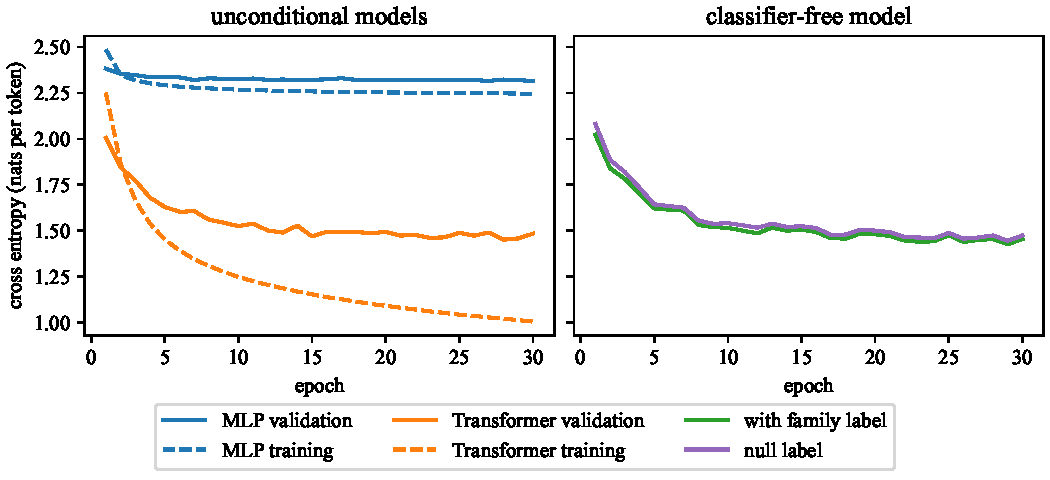
\includegraphics[width=\textwidth]{figures/learning_curves}
  \caption{Cross entropy per epoch, training dashed and validation solid. The right panel evaluates the conditional model twice, once with the family label and once with the null label.}
  \label{fig:curves}
\end{figure*}

\begin{figure*}[t]
  \centering
  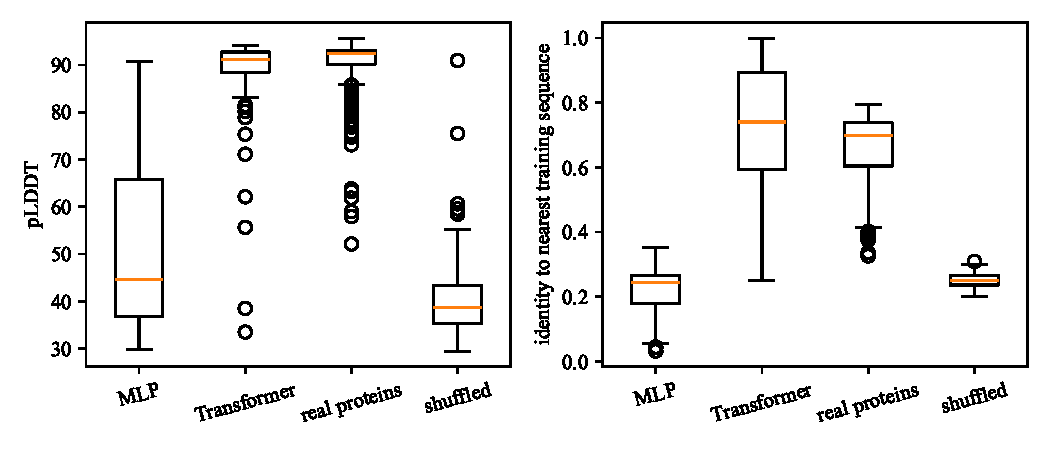
\includegraphics[width=\textwidth]{figures/generation_quality}
  \caption{pLDDT and identity to the nearest training sequence, for the two unconditional models and the two controls. The transformer column uses the 100 unguided samples, the other three 256 each.}
  \label{fig:quality}
\end{figure*}

\begin{figure*}[t]
  \centering
  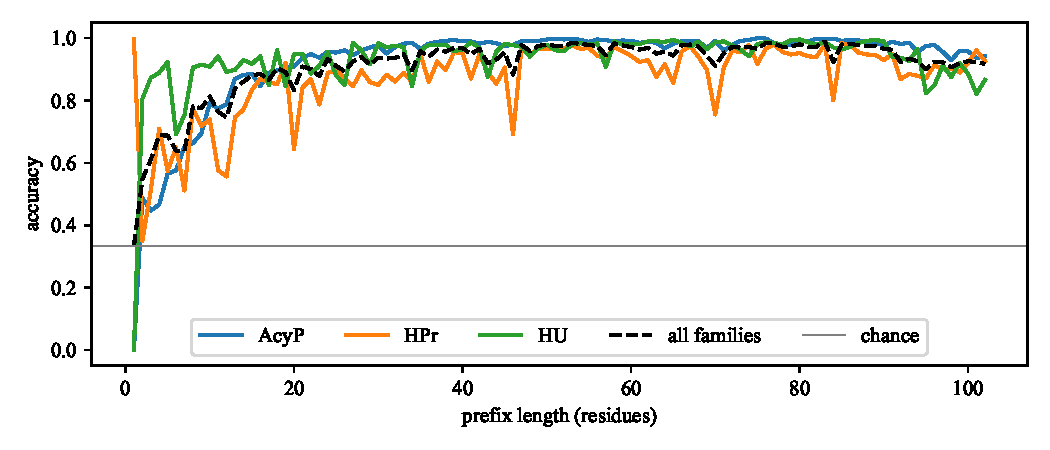
\includegraphics[width=\textwidth]{figures/prefix_accuracy}
  \caption{Accuracy of the classifier head against prefix length, per family and over all three. Positions where fewer than 300 validation sequences remain are left out, which ends the curve at 102 residues.}
  \label{fig:prefix}
\end{figure*}

\begin{figure*}[t]
  \centering
  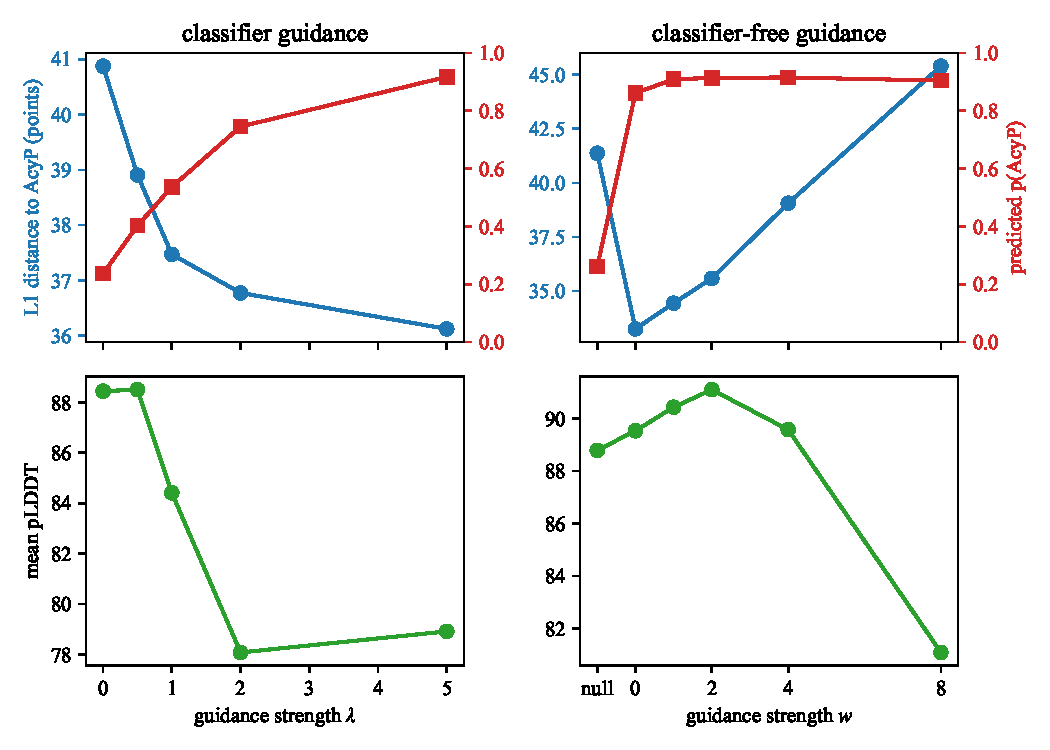
\includegraphics[width=\textwidth]{figures/tradeoff}
  \caption{Guidance strength against family membership and structural plausibility, classifier guidance in the left column and classifier-free guidance in the right. The upper panels carry two scales, composition distance in blue and predicted membership in red. The null label run has no $w$ and sits at the left edge.}
  \label{fig:tradeoff}
\end{figure*}

\begin{figure*}[t]
  \centering
  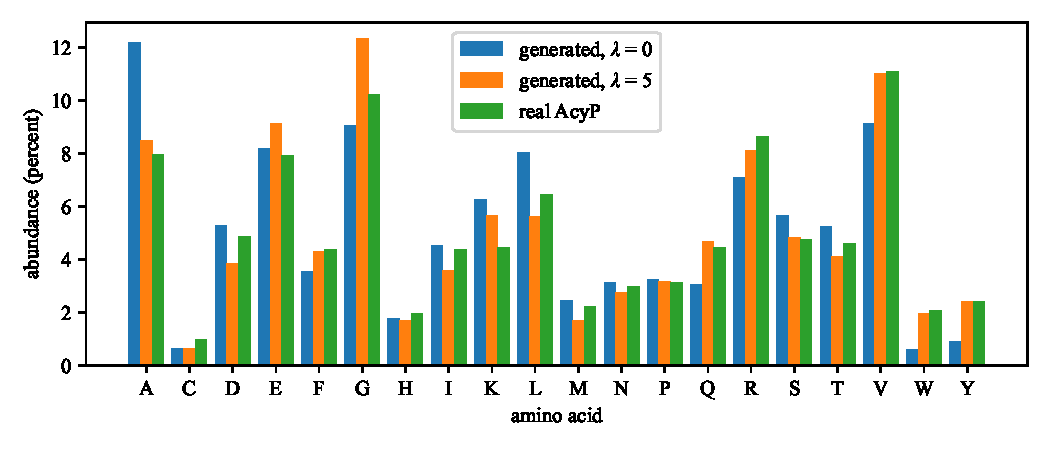
\includegraphics[width=\textwidth]{figures/composition_profile}
  \caption{Mean amino acid composition of the guided samples at $\lambda = 0$ and $\lambda = 1$, next to the AcyP mean of the training set. 100 sequences per setting.}
  \label{fig:composition}
\end{figure*}

\end{document}
